\chapter{ Resultados Experimentais }
\label{cap:resultados}
\section{Experimentos}




\subsection{Modelos Simples de Aprendizado de Máquina}

Para esses modelos como Redes Neurais, Árvores de Decisão e Regressões
Lineares, separamos os dados em treino e validação, normalizamos as variáveis e
treinamos os modelos. 

\subsubsection{Divisão dos dados entre treino e validação}


A divisão entre dados de treino e validação é feita da maneira padrão com
modelos de Aprendizado de Máquina, separando-se $80\%$ dos dados para treino e
$20\%$ para validação, i.e. testar o poder de generalizacão dos modelos. 

\begin{figure}[H]
  \centering
  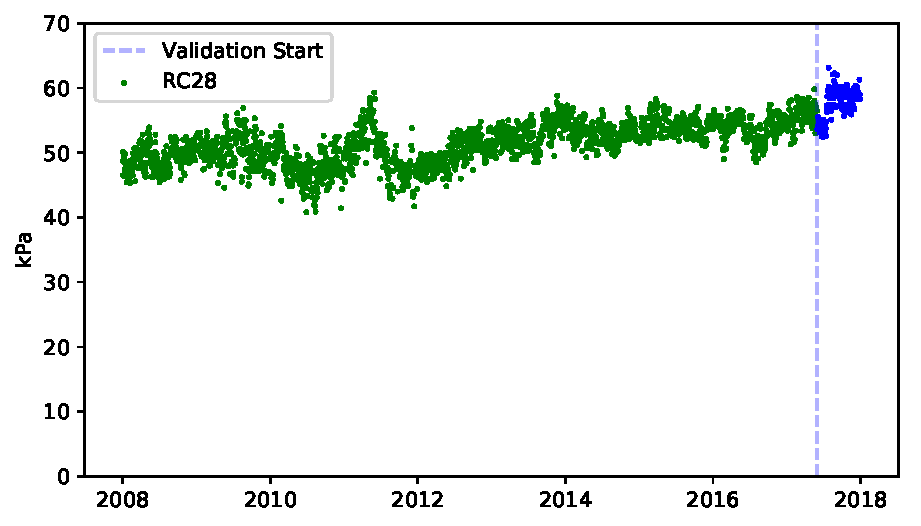
\includegraphics[width=0.9\columnwidth]{train_dev.pdf}
  \caption{Divisão do dataset para a saída RC28, os pontos verdes foram usados para
    treino e os pontos azuis usados para validação.}
  \label{fig:divrc28}
\end{figure}

Foram usadas implementacões dos modelos fornecidos pela biblioteca Sklearn.
As avaliações de RMSE de todo o conjunto de validação estão apresentados por modelos na Imagem~\ref{fig:linmodels}  

\begin{figure}[H]
  \centering
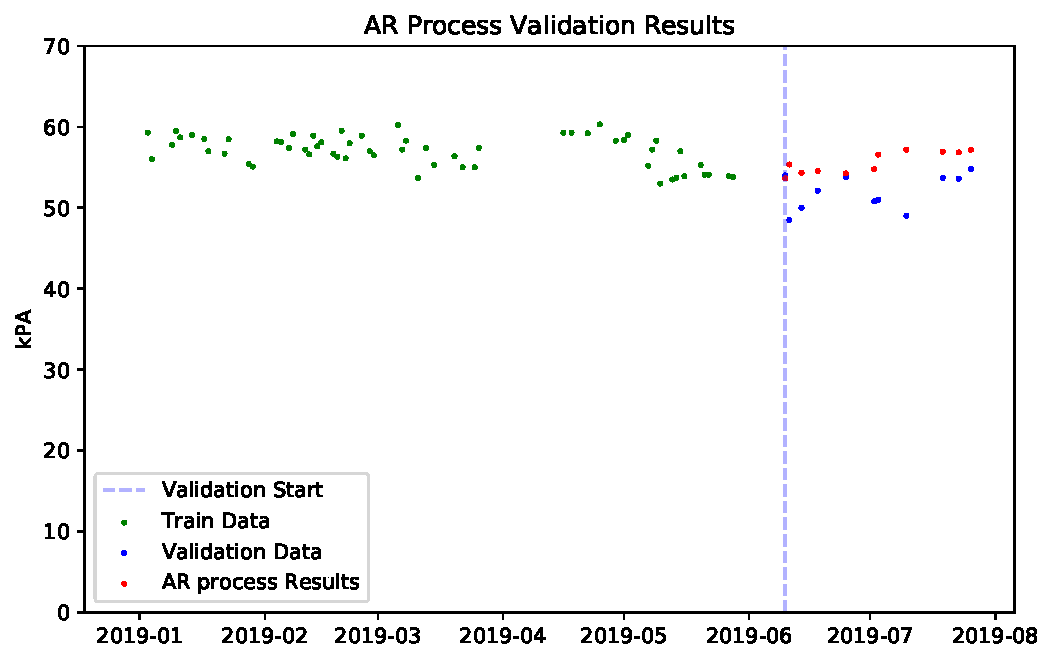
\includegraphics[width=0.9\columnwidth]{linear_exp.pdf}
\caption{Predições nos dados de validação nos experimentos com modelos não-temporais. }
\label{fig:linmodels}
\end{figure}

Na Tabela~\ref{tb:rmse_lin} reportamos os erros para predições imediatamente
após o fim do último dia de dados usados para treino. Iremos mostrar o
erro para o dia seguinte, três dias depois e então uma semana após o último dia
de dados usados para treinamento.

\begin{center}
\begin{table}[htbp]
\caption{RMSE values by forecast span}
\centering
\begin{tabular}{rr}
\hline
 Regressão Linear & RMSE\\
\hline
24h & 2.94\\
3d & 0.13\\
7d & 5.43\\
\hline
Rede Neural & RMSE\\
\hline
24h & 3.70\\
3d & 1.26\\
7d & 6.04\\
\hline
Random Forest & RMSE\\
\hline
24h & 1.61\\
3d & 1.36\\
7d & 5.83\\
\end{tabular}

\label{tb:rmse_lin}
\end{table}
\end{center}

 Reportamos distribuição dos valores previstos, até 1 mês após a data
onde começam os dados de validação (i.e. os dados não usamos para treinamento), a Imagem \ref{fig:distr_lin} permite comparar as distribuições previstas pelos 3 modelos:

\begin{figure}[H]
\label{fig:distr_lin}
\centering
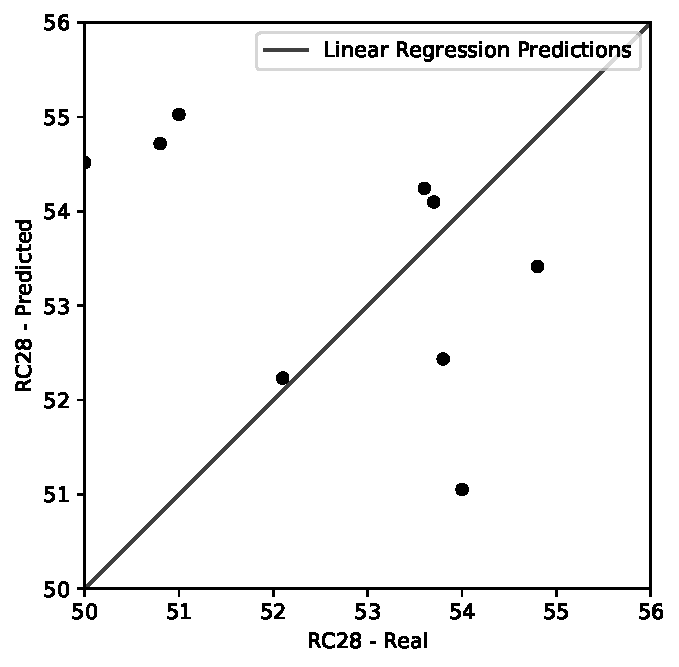
\includegraphics[width=.3\textwidth]{qq-LinearRegression.pdf} \hfill
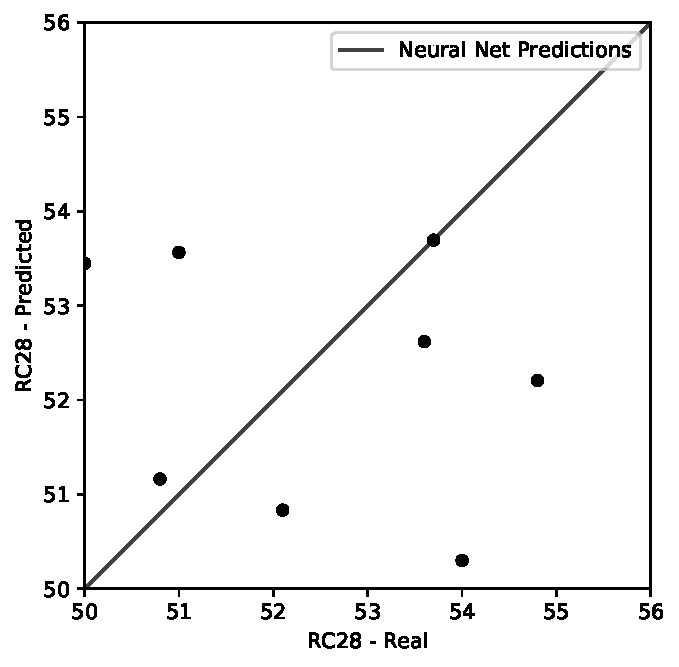
\includegraphics[width=.3\textwidth]{qq-NeuralNet.pdf} \hfill
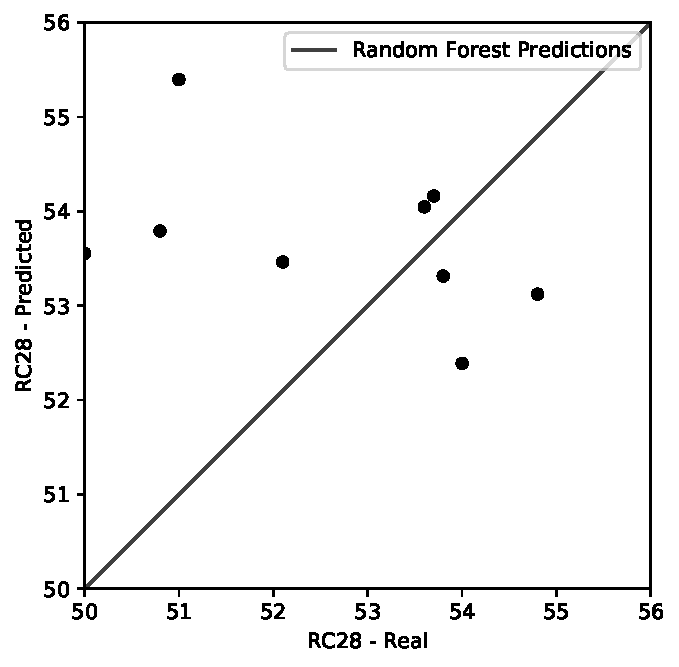
\includegraphics[width=.3\textwidth]{qq-RandomForest.pdf} 
\caption{Valores reais plotados contra os valores previstos para análise da distribuição aprendida por cada modelo} 
\end{figure}

Para modelagem de séries temporais, é comum se estudar o resíduo das
predições. É assumido em uma tarefa de regressão que o resíduo é distribuído
normalmente e com média zero.

\begin{figure}[H]
  \label{fig:res_lin}
  \centering
  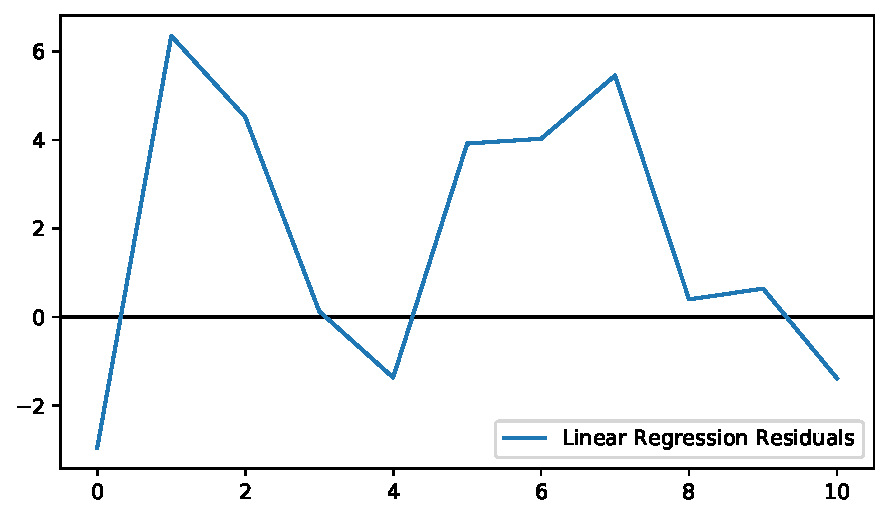
\includegraphics[width=.3\textwidth]{residuals-LinearRegression.pdf} \hfill
  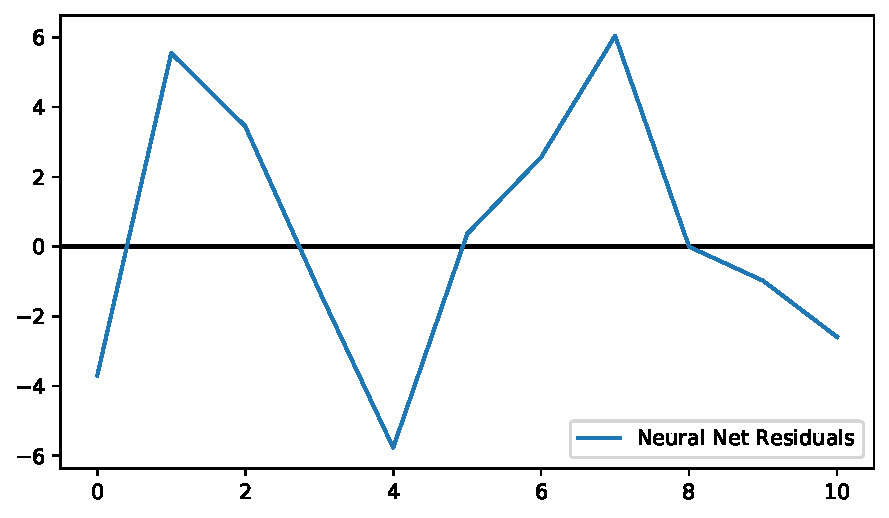
\includegraphics[width=.3\textwidth]{residuals-NeuralNet.pdf} \hfill
  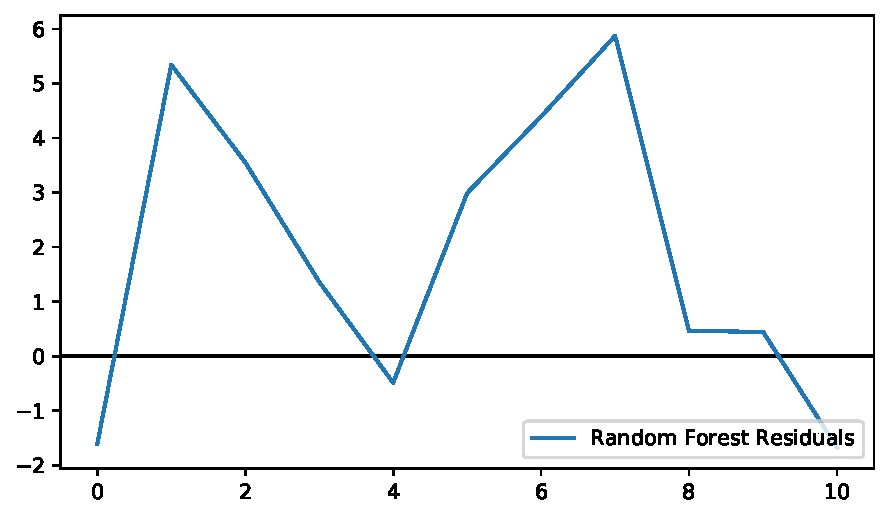
\includegraphics[width=.3\textwidth]{residuals-RandomForest.pdf} 
  \caption{Distribuição dos Erros de cada modelo. Como esperado, todos os erros flutuam em torno da média 0. } 
\end{figure}

\subsection{Modelos para Séries Temporais}


Agora com um tratamento completo do problema como o de previsão de séries
temporais, consideramos os dados sequencialmente, treinando e testando o modelo a partir de janelas de $w$
entradas consumidas em sequência pelo o modelo. A tarefa destes é então gerar
predições que continuem essa janela de dados. Em uma situação real daríamos
alguns dias de dados como entrada e calcularíamos a medida alvo para os próximos dias. 


Como mencionado na introdução desse trabalho, um benefício das técnicas de
Aprendizado Profundo é a de escalar tarefas de aprendizado para datasets de
tamanho muito maior que era possível com modelos clássicos \citep{dlbook}.
Para tarefas de regressão de séries temporais, modelos recentes de Aprendizado
Profundo permitem que sejam usadas diversas séries temporais para a tarefa de
aprendizado. Os modelos poderão então ter parâmetros tanto locais (calculados
para cada série) como globais (dividimos por todas as séries de treinamento).

\subsubsection{Divisão dos dados entre treino e validação}

Com o fim de explorar essa capacidade dos modelos de consumirem diversas séries
temporais, os dados da fábrica de Cajati foram separados por ano e consideramos
cada ano como um exemplo do processo a ser modelado, fornecendo-os separadamente
aos modelos. Os modelos de Aprendizado
Profundo irão então usar parametros locais para cada ano de produção de cimento,
mas globalmente buscar padrões para o funcionamento da fábrica. 

Para cada ano de 2009 até 2019 usaremos os primeiros 11 meses como dados de
treinamento e os últimos 30 dias como dados de validação.



\begin{figure}[H]
  \centering
  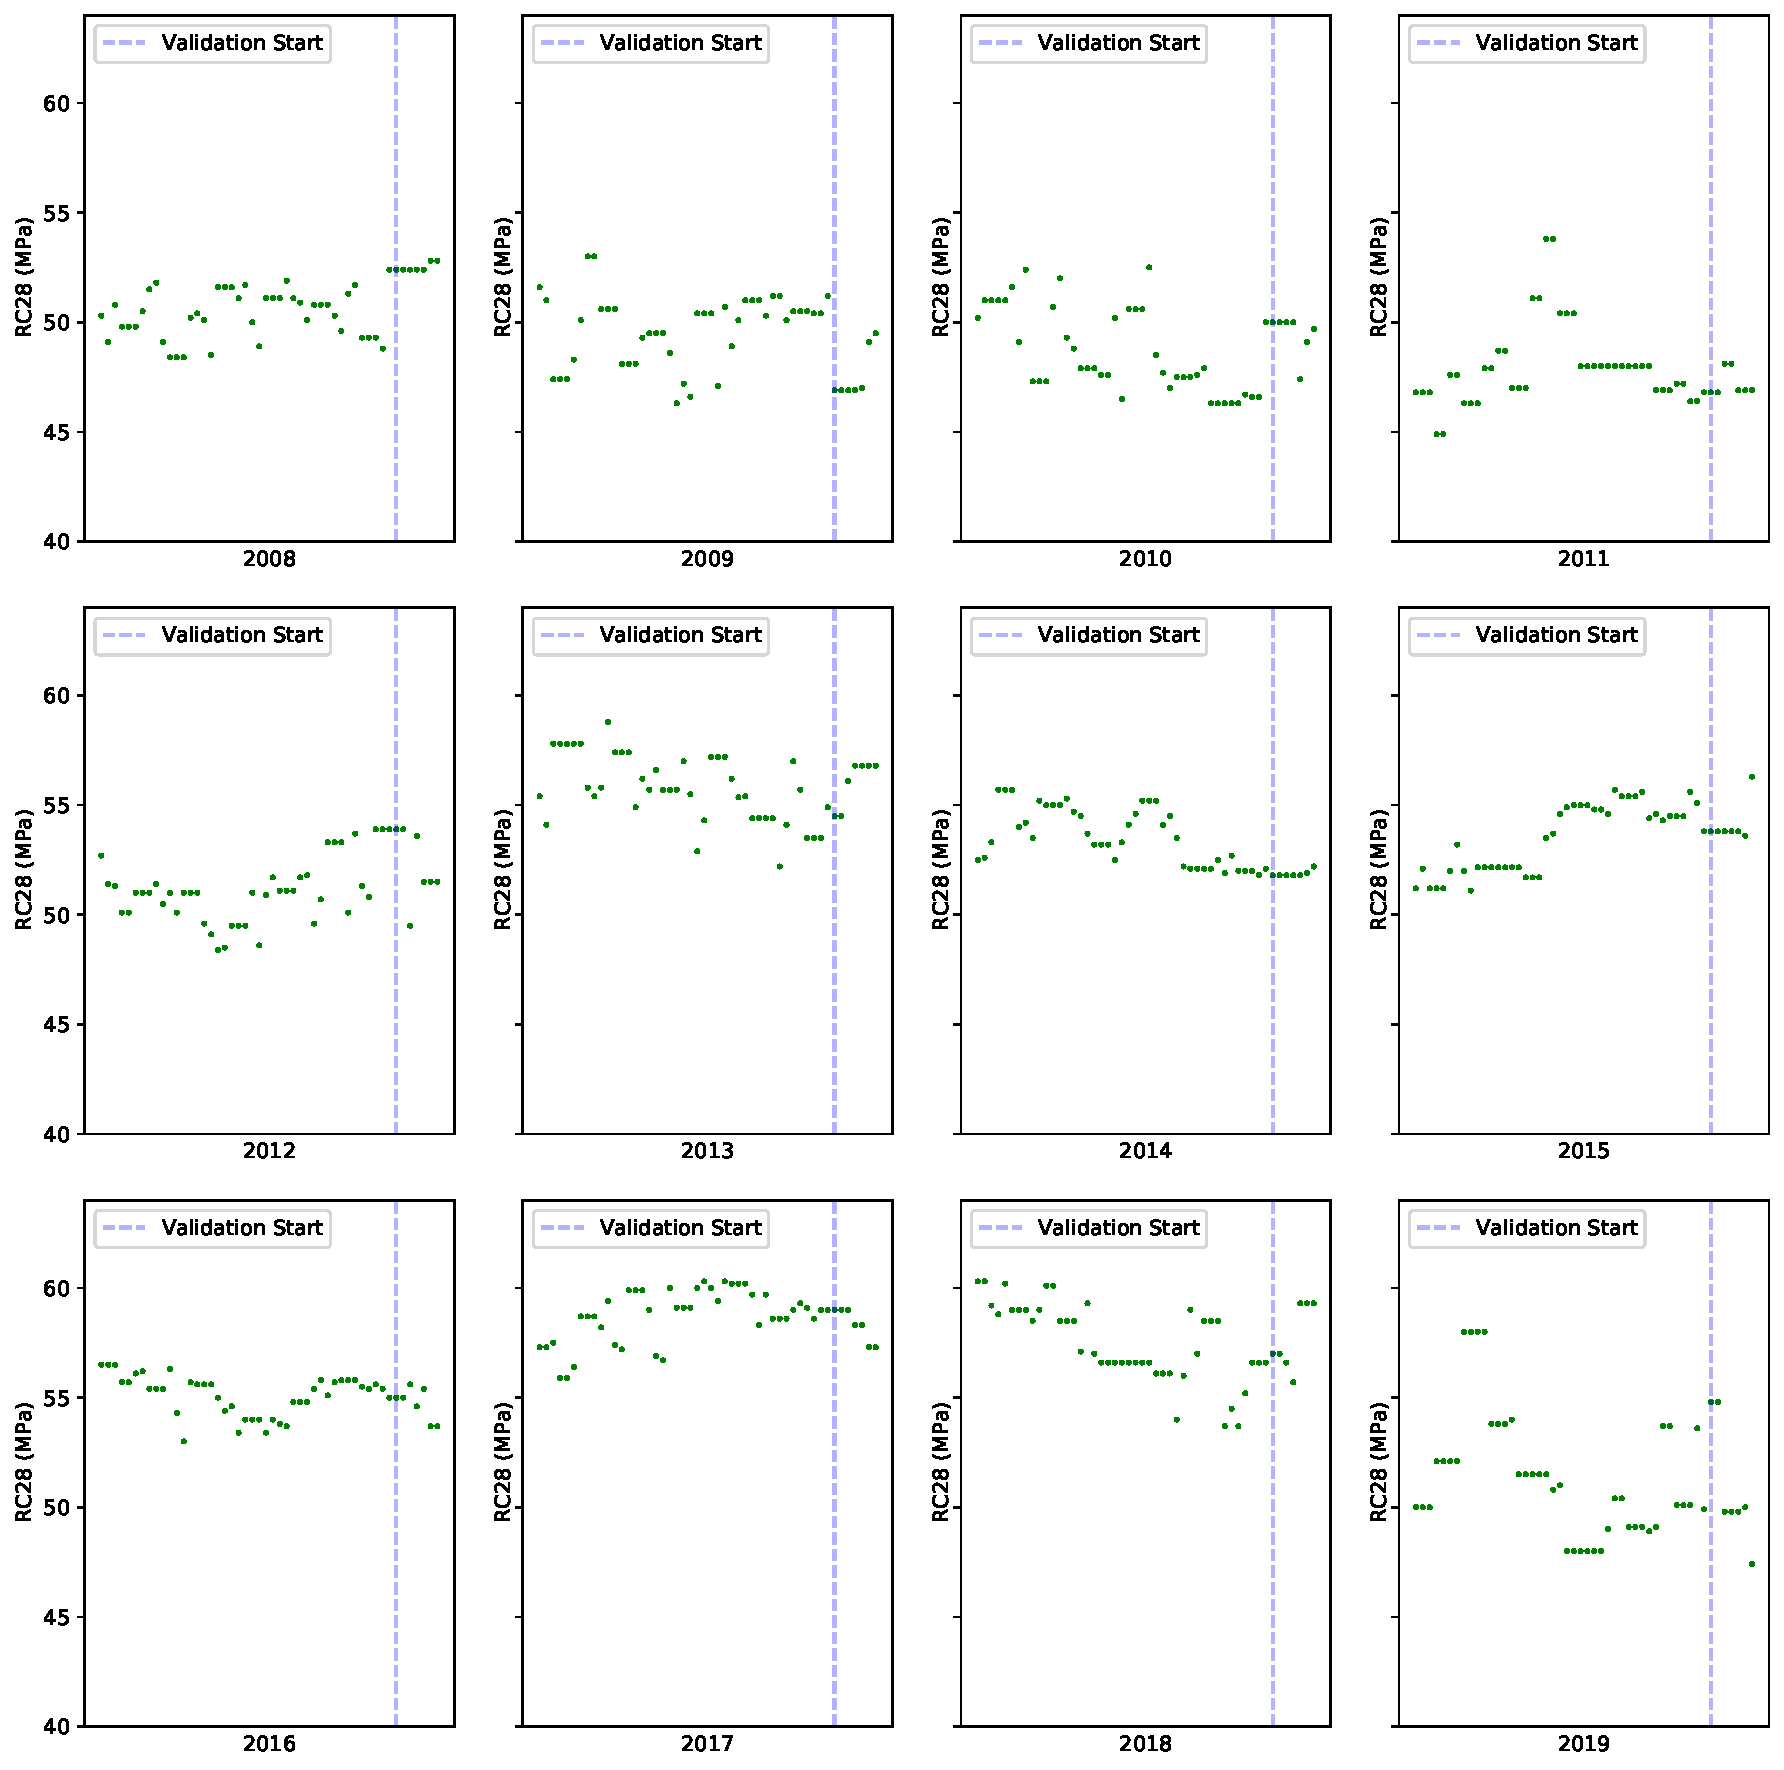
\includegraphics[height=.99\textwidth]{train_val_all_years.pdf} 
  \caption{Os dados são divididos em 11 datasets separados, onde temos por
    dataset 11 meses usados para treino e os últimos dias do ano para validação.} 
  \label{fig:trainvalallyears}
\end{figure}

\subsection{Regressão Linear Dinâmica com Filtragem Exponencial}

Com o fim de termos uma baseline com a qual compararmos os modelos de Deep
Learning, aplicaremos o modelo proposto em \citep{grecialin}.
Para tal criamos as janelas de dados de treinamento e teste
como explicado anteriormente nesse trabalho.  

Usaremos 3 modelos com diferentes grupos de variáveis, a tabela a seguir mostra
as variáveis presentes em cada modelo, e o nome dado aos modelos pelo restante
desse trabalho. Também mostraremos resultados para o modelo corrigido
reglin\_ew, que é uma combinação dos modelos reglin\_1 e reglin\_7.


% copiar output do pandas aqui
% esta no notebook papergrecia
\begin{table}[]
\centering 
\begin{tabular}{llllllllllllll}
\toprule
reglin\_1 &  AGP &  AL2O3 &  SIO2 &  MGO &  IP &  FP &  SBL &  PF &  P2O5 &  FE2O3 &  RC1 &      &      \\
reglin\_3 &  AGP &  AL2O3 &  SIO2 &  MGO &  IP &  FP &  SBL &  PF &  P2O5 &  FE2O3 &  RC1 &  RC3 &      \\
reglin\_7 &  AGP &  AL2O3 &  SIO2 &  MGO &  IP &  FP &  SBL &  PF &  P2O5 &  FE2O3 &  RC1 &  RC3 &  RC7 \\
\bottomrule
\end{tabular}
\caption{O conjunto de variáveis usado para cada um dos modelos, de maneira análoga ao apresentado no trabalho \cite{grecialin}}
\label{tab:modelslin}
\end{table}

Os resultados para cada modelo no período de validação de cada ano são reportados a seguir:

\begin{figure}[H]
  \centering
  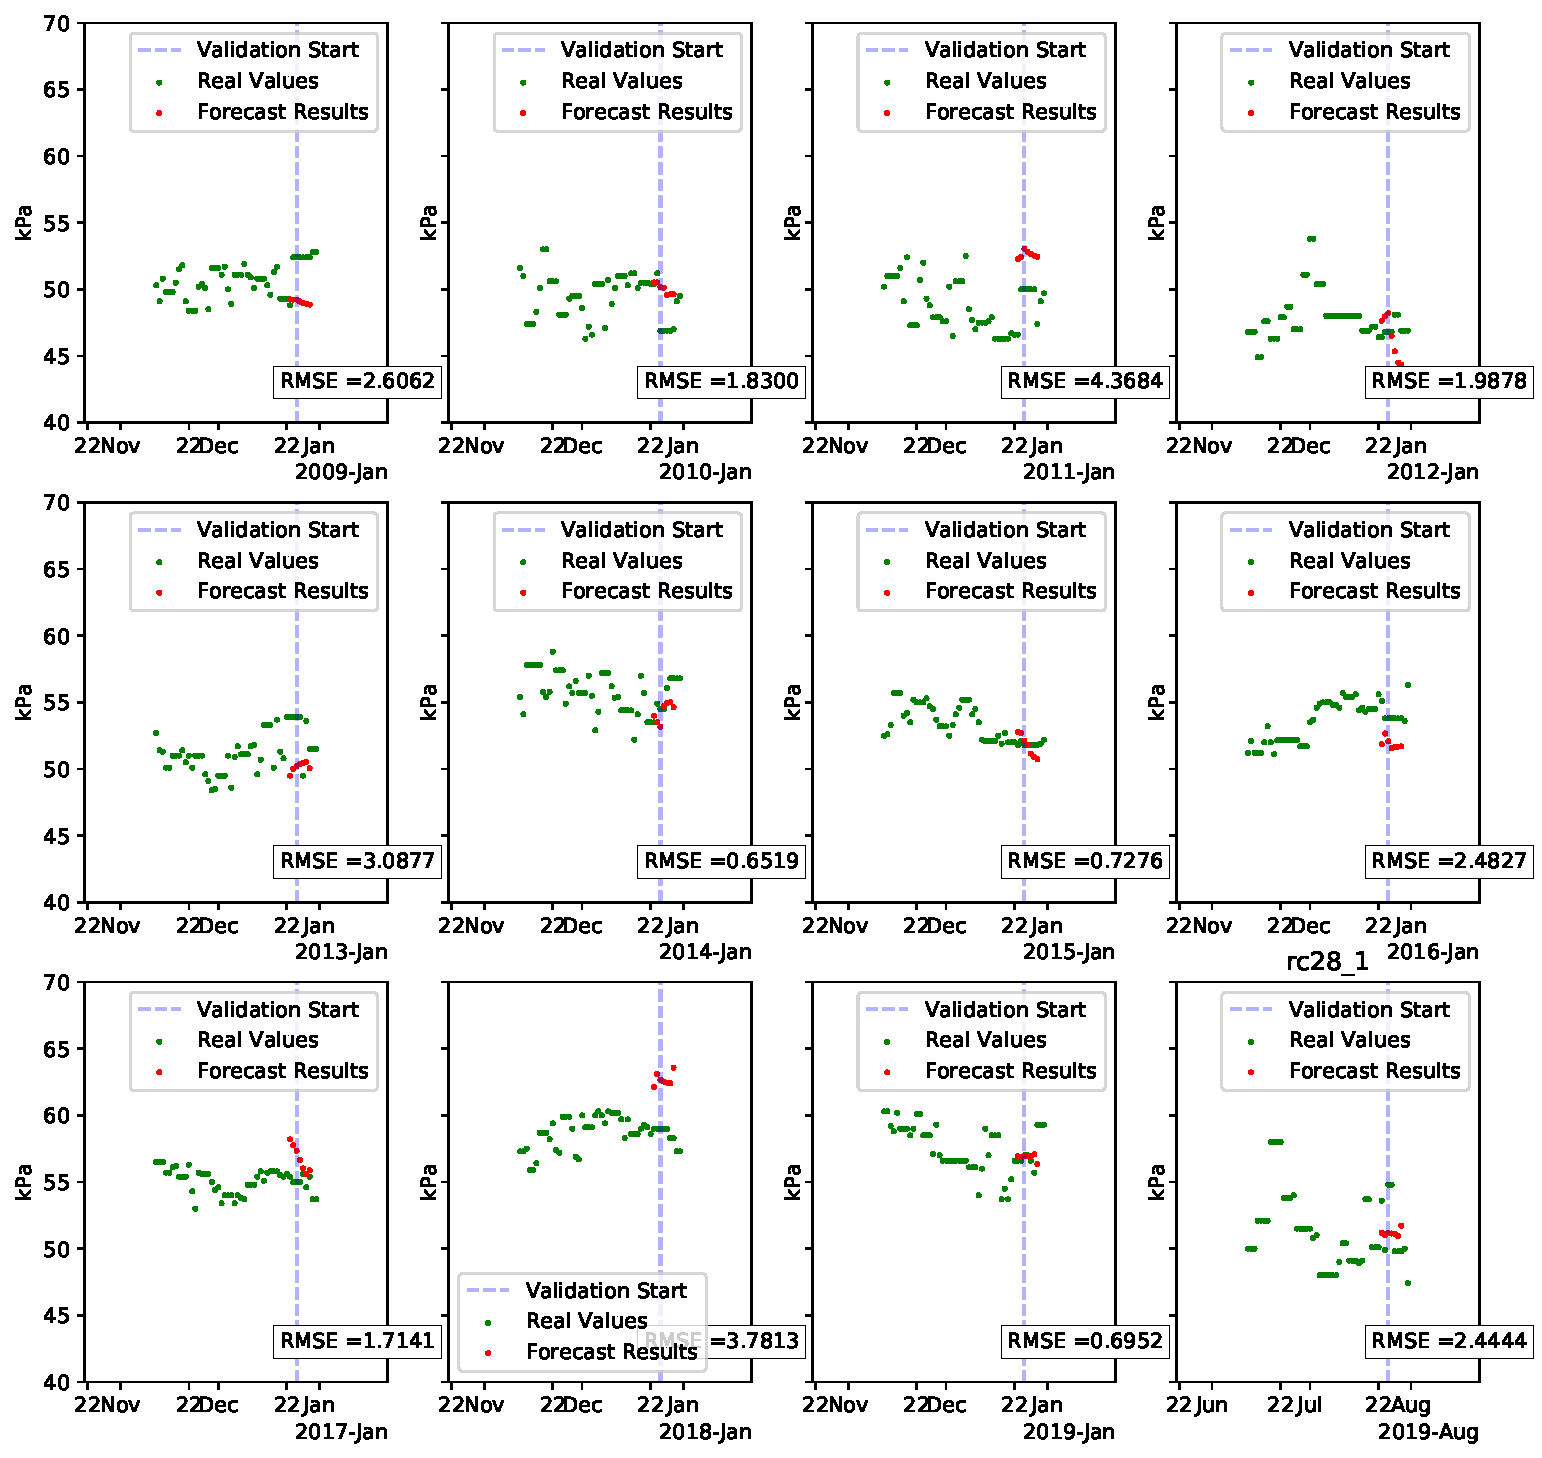
\includegraphics[width=0.9\columnwidth]{predgrecialin-rc28_1.pdf}
  \caption{Predições no período de teste para cada período de validação pelo
    modelo reglin\_1}
  \label{fig:rc281preds}
\end{figure}

\begin{figure}[H]
  \centering
  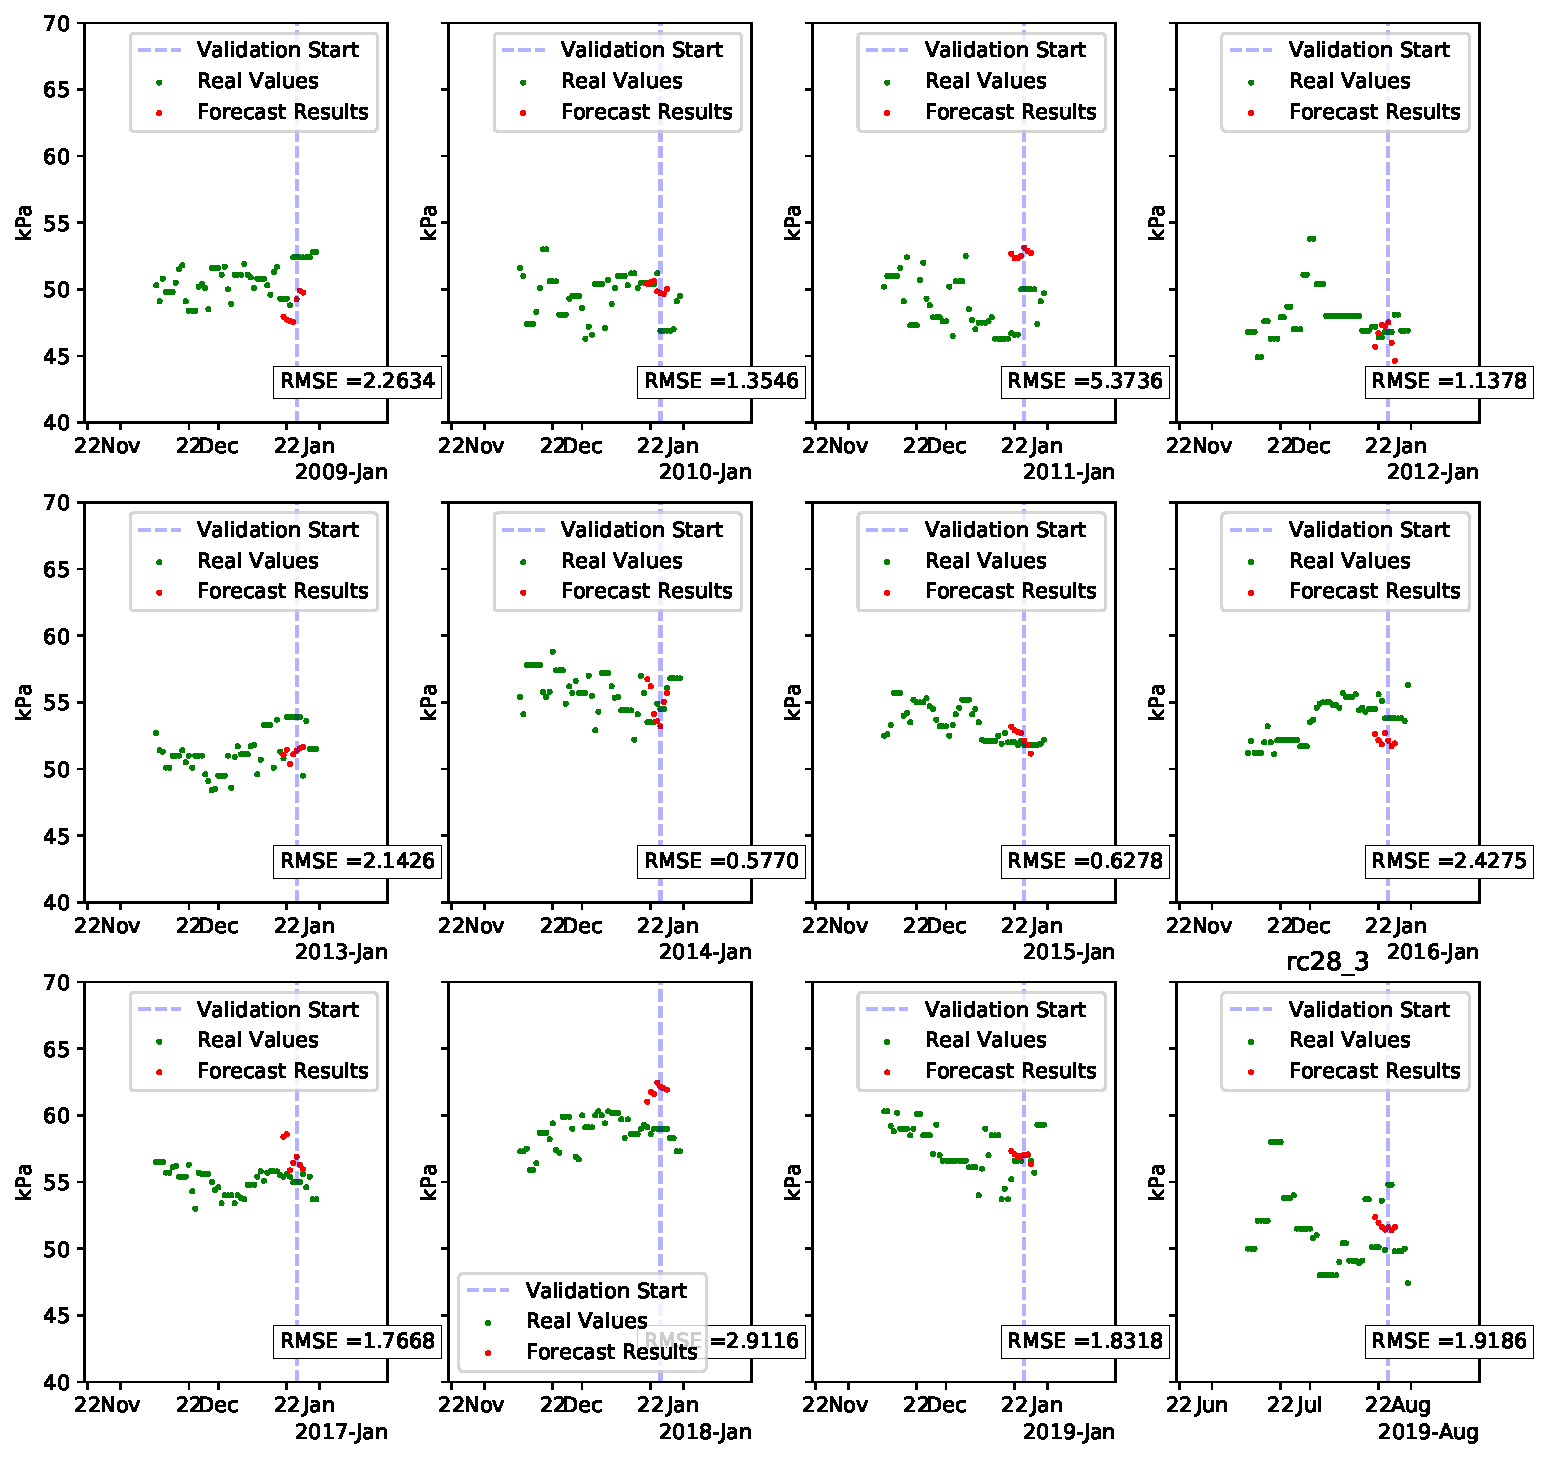
\includegraphics[width=0.9\columnwidth]{predgrecialin-rc28_3.pdf}
  \caption{Predições no período de teste para cada período de validação pelo
    modelo reglin\_3}
  \label{fig:rc281preds}

\end{figure}
\begin{figure}[H]
  \centering
  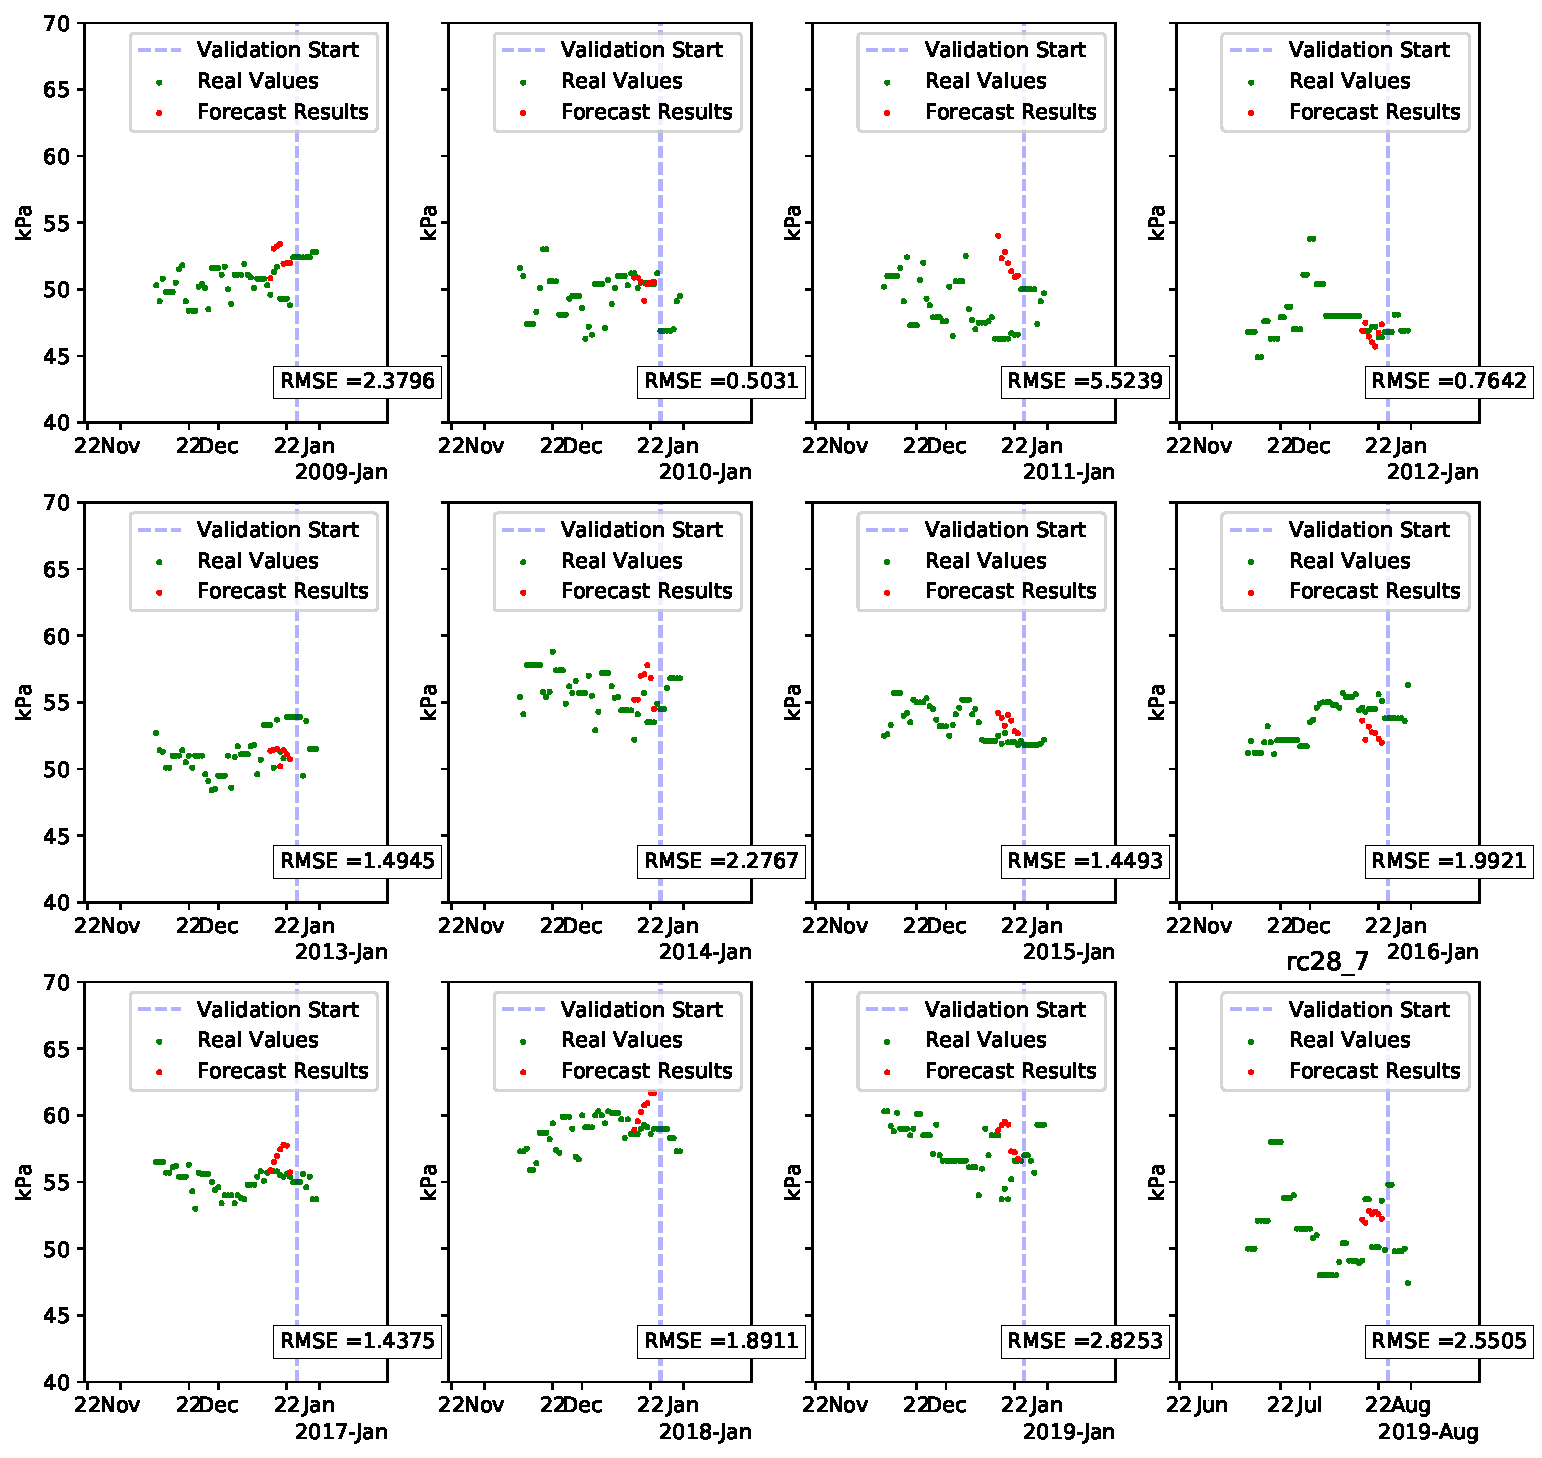
\includegraphics[width=0.9\columnwidth]{predgrecialin-rc28_7.pdf}
  \caption{Predições no período de teste para cada período de validação pelo
    modelo reglin\_7}
  \label{fig:rc281preds}

\end{figure}

Agregando esses valores, podemos apresentar o RMSE médio para cada modelo para
todo o dataset, para predições de 24h e 7 dias.

\begin{center}
  \begin{table}[]
    \centering
    \begin{tabular}{l|llll}
      \cline{2-3}
      & \multicolumn{1}{l|}{RMSE 24h} & \multicolumn{1}{l|}{RMSE 7 dias} &  \\ \cline{1-3}
      \multicolumn{1}{|l|}{reglin\_1} & 1.66                          & 2.19                             &  \\ \cline{1-1}
      \multicolumn{1}{|l|}{reglin\_3} & 2.12                          & 2.02                             &  \\ \cline{1-1}
      \multicolumn{1}{|l|}{reglin\_7} & 2.09                          & 1.63                             &  \\ \cline{1-1}
      \multicolumn{1}{|l|}{reglin\_ew} & 2.12                          & 1.42                             &  \\ \cline{1-1}
    \end{tabular}
    \caption{Valores agregados de RMSE para os modelos de Regressão Linear Dinâmica}

    \label{tb:rmse_exp}
  \end{table}
\end{center}



\subsection{Modelos de Deep Learning Bayesianos}

\subsubsection{DeepAr}

Usamos a implementação do modelo DeepAR da bibliteca GluonTS \citep{gluonts}. Separamos as variáveis para treinarmos 3 modelos distintos da mesma maneira
apresentada na Tabela~\ref{tab:modelslin}. Esses modelos serão chamados de \textbf{DeepAR\_1}, \textbf{DeepAR\_3} e \textbf{DeepAR\_7}. 
As Figuras~\ref{fig:fordeepar1},\ref{fig:fordeepar3} e \ref{fig:fordeepar7} reportam as
predições geradas em cada dataset de treino por cada modelo. Também corrigimos o
modelo \textbf{DeepAR\_1} com o modelo \textbf{DeepAR\_7} de maneira análoga a
Sessão~\ref{ses:ewma}, ao modelo corrigido damos o nome de \textbf{DeepAR\_ew}. 

\begin{figure}[H]
  \centering
  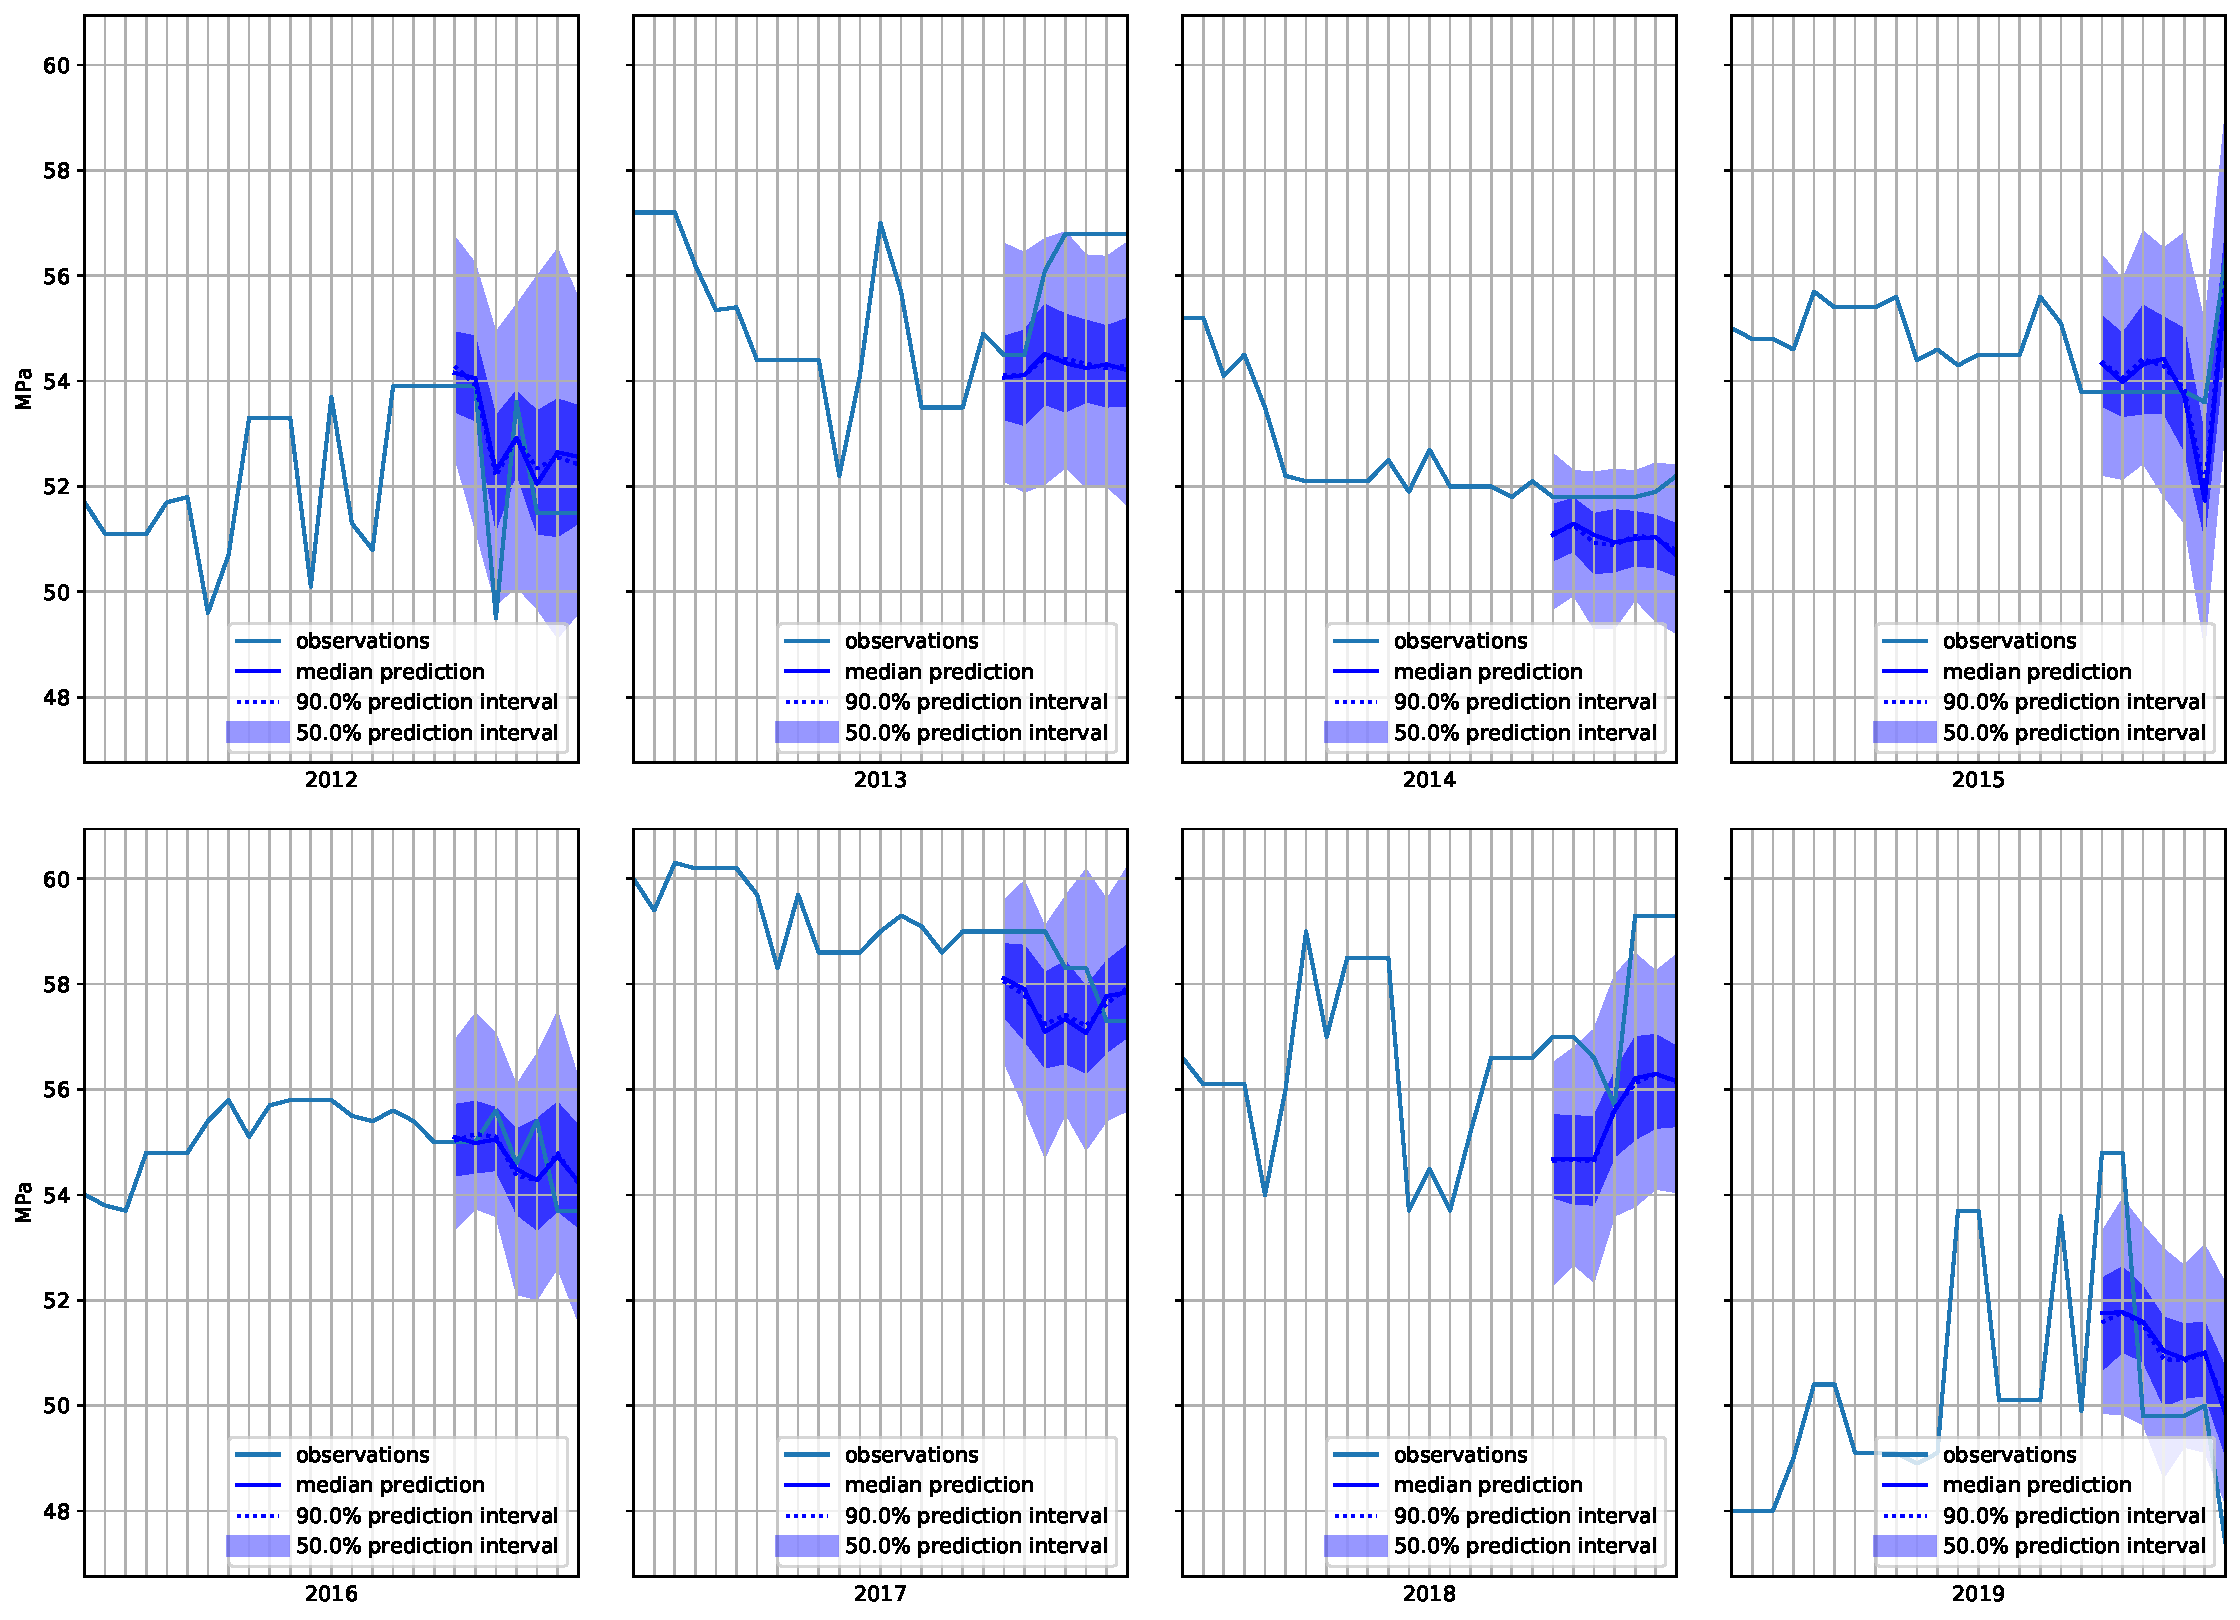
\includegraphics[width=.99\textwidth]{forecast_deep_ar1.pdf} 
  \caption{Predição para todos os dados de validação para o modelo DeepAR\_1}
  \label{fig:fordeepar1}
\end{figure}

\begin{figure}[H]
  \centering
  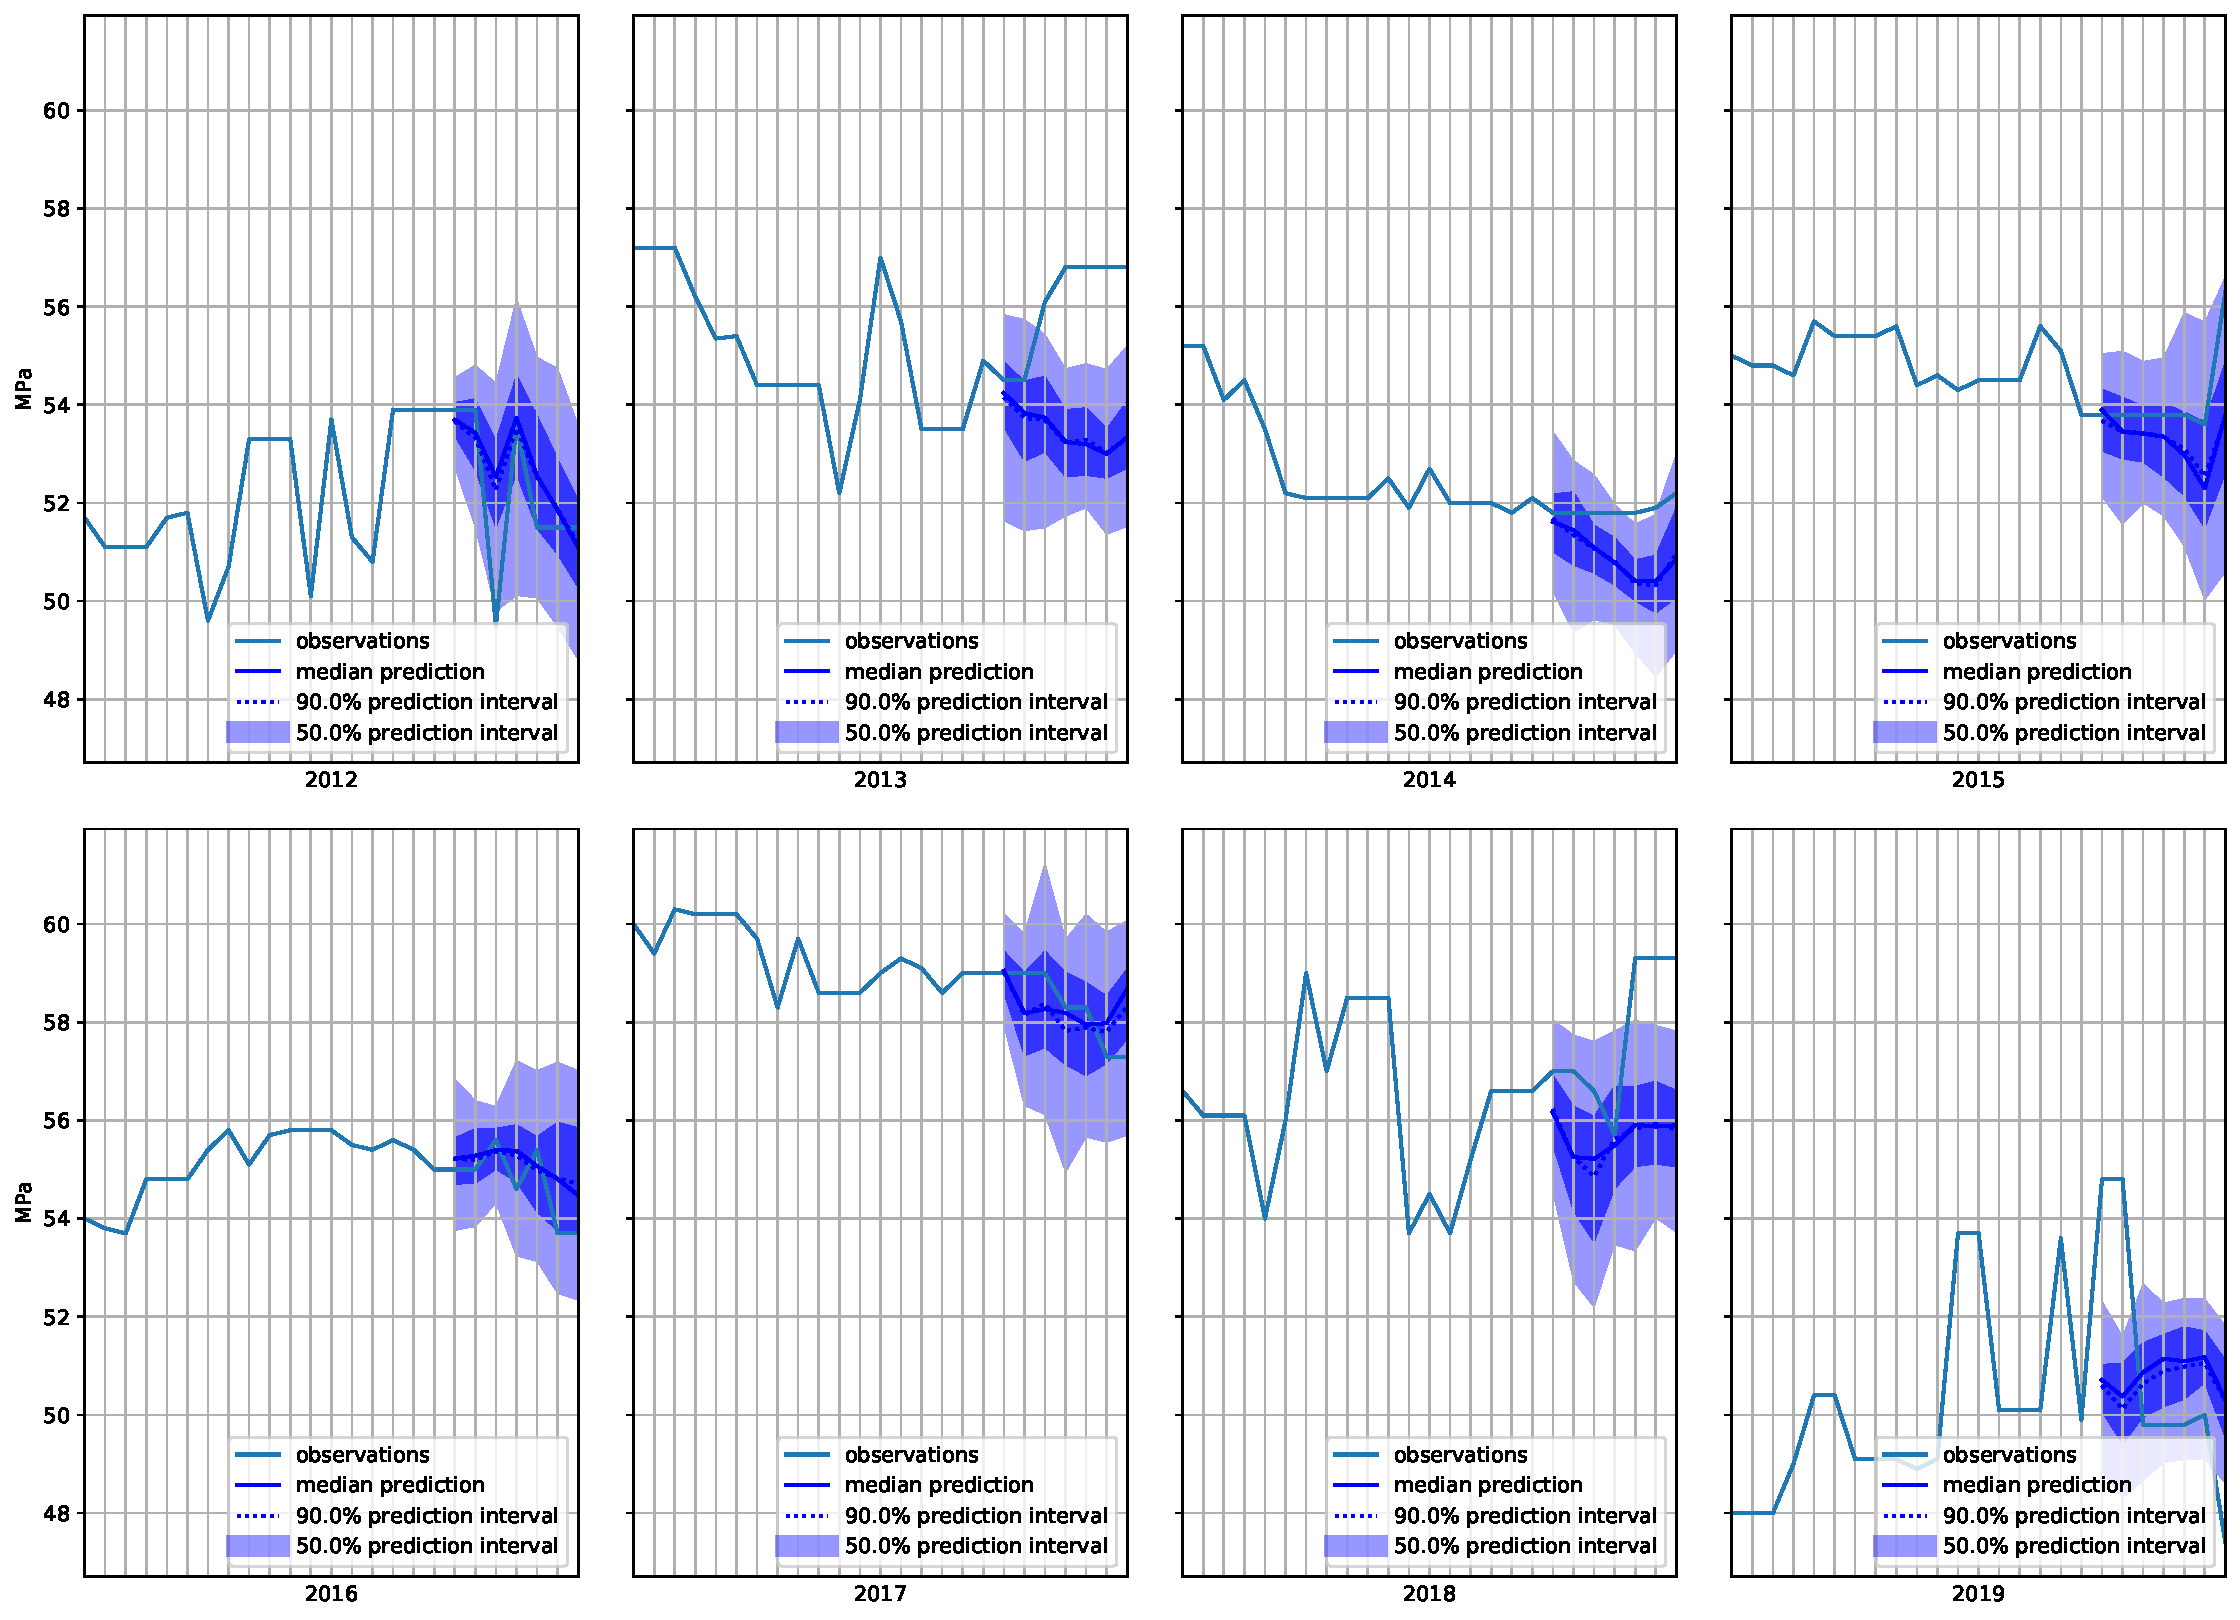
\includegraphics[width=.99\textwidth]{forecast_deep_ar3.pdf} 
  \caption{Predição para todos os dados de validação para o modelo DeepAR\_3}
  \label{fig:fordeepar3}
\end{figure}

\begin{figure}[H]
  \centering
  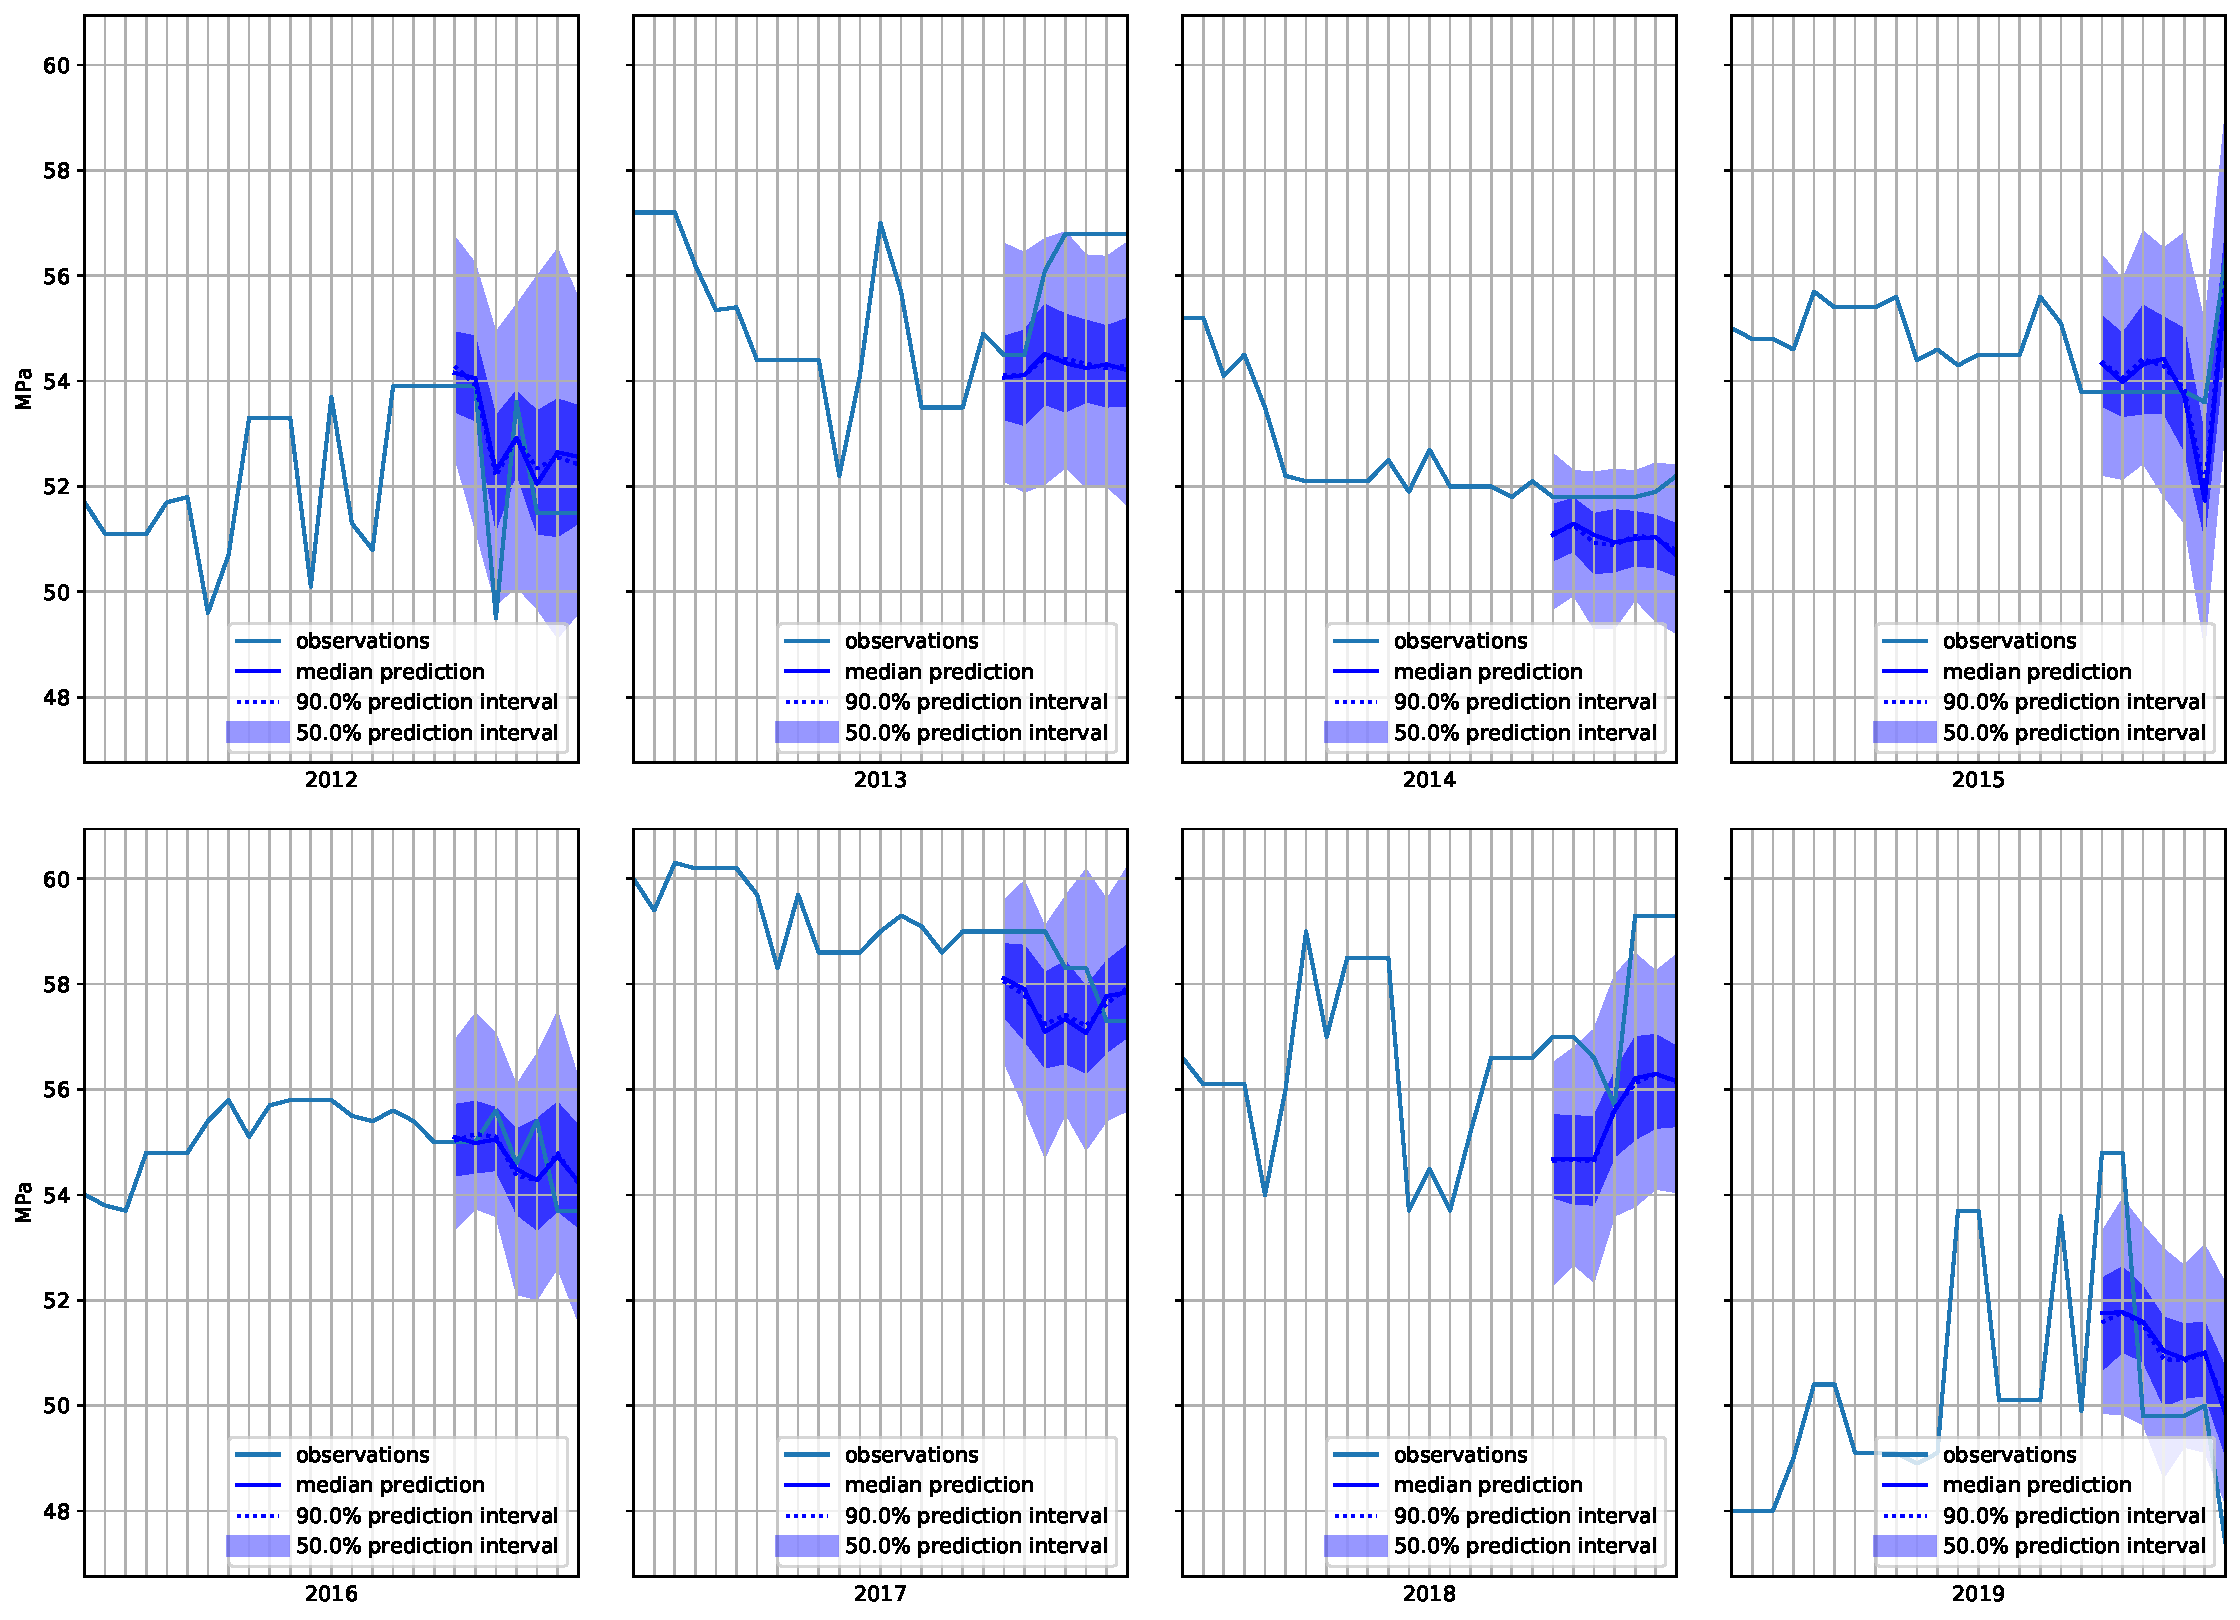
\includegraphics[width=.99\textwidth]{forecast_deep_ar7.pdf} 
  \caption{Predição para todos os dados de validação para o modelo DeepAR\_7}
  \label{fig:fordeepar7}
\end{figure}


A Tabela~\ref{tb:rmsedeepar} agrega os resultados do modelo DeepAR, para cada
conjuntos de variáveis. Comparando esses resultados com os obtidos pelo modelo
linear dinâmico. Os modelos DeepAR consistentemente geram melhores predições agregando valores previstos por 7 dias
após a implementação do modelo em produção. As predições de 24h são naturalmente
ruidosas para todos os modelos testados nesse trabalho.

\begin{center}
\begin{table}[]
  \centering
  \begin{tabular}{l|llll}
    \cline{2-3}
    & \multicolumn{1}{l|}{RMSE 24h} & \multicolumn{1}{l|}{RMSE 7 dias} &  \\ \cline{1-3}
    \multicolumn{1}{|l|}{reglin\_1/DeepAR\_1} & 1.66 / 1.68                   & 2.19 / 1.75                      &  \\ \cline{1-1}
    \multicolumn{1}{|l|}{reglin\_3/DeepAR\_3} & 2.12 / 1.86                   & 2.02 / 1.68                      &  \\ \cline{1-1}
    \multicolumn{1}{|l|}{reglin\_7/DeepAR\_7} & 2.09 / 1.82                   & 1.63 / 1.42                      &  \\ \cline{1-1}
    \multicolumn{1}{|l|}{reglin\_ew/DeepAR\_ew} & 2.12/ 1.16                   & 1.42 / 1.12                      &  \\ \cline{1-1}
  \end{tabular}
  \caption{Valores do RMSE para cada modelo nos horizonte de predição de 24h e 7 dias.}
\label{tb:rmsedeepar}
\end{table}
\end{center}
